\chapter{Measuring similarity}
\label{ch:background}

In this chapter, we provide an overview of the theoretical background of many
methods we employed to solve our problem. As \enquote{finding similar
neighborhoods} implies, the underlying theme is measuring similarity between
objects. This can be used to cluster them in meaningful groups
(\autoref{sec:clustering}). An important step is to tailor general metric
toward our goal (\autoref{sec:metric}). Indeed, \textcite{GoodSimilarity08}
show that \enquote{good} properties of similarity functions are transferred to
classifiers using them.

\section{Clustering}
\label{sec:clustering}

A general class of methods addressing unsupervised problems is clustering.
\enquote{\emph{Clustering algorithms partition a given data set into several
groups based on some notion of similarity between objects}}
\autocite{LimitsClustering05}. The most widely used is the
\methodname{$k$-means algorithm} \autocite{kmeans67}. After initially choosing
$k$ centroids, an iterative process takes place, divided in two phases. First
each point is assigned to the cluster of the closest centroid. Then centroids
positions are updated by taking the mean of all points belonging to their
cluster. Convergence occurred when centroids positions do not change between
iterations. In practice, the algorithm is fast but it is only guaranteed to
find a local optimal of the within-cluster sum of squares: \[ \sum_{i=1}^{k}
\sum_{ x_j \in S_i} \left\| x_j - \mu_i \right\|^2 \] Another drawbacks is that
$k$, the number of clusters, has to be specified before algorithm execution,
whereas this information is often unknown at this stage. Finally, because it
results in a Voronoy diagram, the clusters found are linearly separable, which
may not reflect the actual data.

Because of these limitations, numerous alternatives have been developed. A
cluster can be defined as an area of high density surrounded by low density
regions. This definition suggests assigning a numeric value of density to every
point of space. A common method is \marginpar{Maybe there is a more practical
reference, especially for multivariate estimation} \methodname{Kernel Density
Estimation} \autocite{KDE56}. Basically, a kernel is centered around each point
(\ie{} a symmetrical weighting function, for instance a Multivariate Gaussian)
and the estimation of the probability distribution $f$ is their normalized sum:
% http://en.wikipedia.org/wiki/Multivariate_kernel_density_estimation
\[ \hat{f}_\bold{h}(\bold{x})= \frac{1}{n} \sum_{i=1}^n K_\bold{h} (\bold{x} -
\bold{x}_i) \]

Yet this does not provide any clustering. One idea would be to find the modes of
$\hat{f}$, which is the underlying principle of Mean Shift
\autocite{MeanShift95}. Another density based algorithm is
\methodname{\textsc{DBSCAN}} \autocite{DBSCAN96}. It has two parameters: a
distance $\epsilon$ and a number of points $\mathrm{minPts}$. A core sample is
a point with at least $\mathrm{minPts}$ neighbors in its
$\epsilon$-neighborhood. From a core sample, its neighbors are visited to find
other core samples belonging to the same cluster. Once it is not more possible,
the algorithm moves to another point. Points that are $\epsilon$ close to a
core sample without having a large enough neighborhood are also part of the
cluster (but are deemed fringe points rather than core ones). Any other
remaining point is noise. With an appropriate index structure (see
\autoref{sub:spatial-structures}), neighborhood queries takes $O(\log n)$ time
and the algorithm runs in $O(n\log n)$. Otherwise, one need to compute the
pairwise distance matrix, which takes $O(n^2)$ time and memory. DBSCAN finds
an arbitrary number of clusters with arbitrary shapes. In the special case where
points carry user identification (like photos or tweets), it can be tweaked to
favor areas that exhibit large user diversity \autocite{PDBSCANKisilevich2010}.
Another extension, OPTICS, can identify clusters despite data having varying
density, but it only produces a reachability-plot, which require further
processing to be transformed into clusters \autocite{OPTICS99}.

\begin{comments}
	I didn't use these methods so I probably don't need to talk about it\\
	Some are based on graphs. For instance \methodname{Spectral
	Clustering} \autocite{SpectralClustering01} (which is related to
	Kernel $k$-means, as shown by \textcite{KernelKmeans04}).
	\methodname{Affinity Propagation} \autocite{AffinityPropagation07}
% https://en.wikipedia.org/wiki/Affinity_propagation
% http://scikit-learn.org/stable/modules/clustering.html#affinity-propagation

	Others are hierarchical
\url{https://en.wikipedia.org/wiki/Hierarchical_clustering}
\end{comments}

A major component of all clustering algorithm is the distance function, and
the space where it operates. The default choice is the Euclidean metric in the
original feature space but these two parameters can be changed. In the latter
case, it often leads to dimensionality reduction.

\subsection{Dimensionality reduction}

Again, there are many methods, but many of them are based on the idea of
preserving distances between points, under the general name Multidimensional
Scaling \autocite{MDS77}. Given points $i$ and $j$ in the original space, we
know their separation $\delta_{i,j}$ with a weight $w_{i,j}$\footnote{that
denotes confidence in the measurement or importance of the points.}. We are
looking for their new position $x_i$ and $x_j$ in the reduced space such that
the stress \[ S = \sum_{i,j} \sqrt{\frac{\sum w_{i,j}(\delta_{i,j} - d(y_i,
y_j))^2}{\sum d(y_i, y_j)^2}} \] is minimized.

Instead of interpreting distances in a geometrical sense, it is also possible
to give them a probabilistic fashion.  Namely, in Stochastic Neighbor Embedding
\autocite{SNE02}, starting from the dissimilarity between two points $i$ and
$j$, $d^2_{ij} = \frac{\vnorm{x_i - x_j}^2}{2\sigma^2_i}$, we compute the
probability of $i$ picking $j$ as a neighbor in the original space \[ p_{ij} =
\frac{\exp(-d_{ij}^2)}{\sum_{k \neq i}\exp(-d_{ik}^2)}\]

We do the same in the low dimensional space, where positions are denoted by
$y_i$ \[ q_{ij} = \frac{\exp(-\vnorm{y_i - y_j}^2)}{\sum_{k \neq
i}\exp(-\vnorm{y_i - y_k}^2)}\] and we set the $y_i$ to minimize $\sum_i
KL(P_i || Q_i)$, which can be understood as preserving the neighborhood of each
point. Later was introduced \tsne{} \autocite{tSNE08}, which makes the
optimization problem simpler and avoid the crowding problem by modeling
distances in the low dimensional space with a heavy tail Student t-distribution
with one degree of freedom \[ q_{ij} = \frac{\left(1+\vnorm{y_i -
y_j}^2\right)^{-1}}{\sum_{k \neq i}\left(1+\vnorm{y_i - y_k}^2\right)^{-1}}\]
An ingenious implementation runs in $O(n\log n)$ \autocite{BarnesHut13}.

It is easier to visually evaluate clustering results in this two or three
dimensional space, although dimensions are not necessarily meaningful.
Furthermore, we assume that sample points are not randomly distributed in the
whole space. Thus, we are trying to recover the low dimensional manifold where
they lie.

\subsection{Spatial data structure}
\label{sub:spatial-structures}

A common subproblem of all the methods exposed so far is to retrieve the $k$
closest neighbors of a given point. If there are $n$ candidates in a $d$
dimensional space, a naive linear scan takes a prohibitive $O(n\cdot d)$ time.
Fortunately, there are data structure well suited to solve this problem faster,
even tough they become less efficient as $d$ increase. Namely, we will describe
$k$-d tree and ball tree. The common idea behind them is to partition space
according to points distribution.

$k$-d tree \autocite{kdtree75}

ball tree \autocite{BallTree89}

We will also mention R-trees \autocite{Rindex84}, which are able to retrieve
more complex geometric shape than point.

\section{Metric}
\label{sec:metric}

\subsection{Ground metric}

Instead of projecting points in a new space, we can directly modify the norm
used to compute distance, that is replace the $L_2$ norm $\vnorm{x-y}_2^2$,
for instance by $L_1$ norm (Manhattan distance) or $L_\infty$. Noting that
$\vnorm{x-y}_2^2 = (x-y)^T A (x-y) = d_A(x,y)$, where $A=I$, one can also
replace $A$ by any positive definite matrix to still define a metric. A well
motivated choice is setting $A$ as the inverse of the covariance matrix,
corresponding to the Mahalanobis distance \autocite{Mahalanobis36}. But $A$
can be learned from the data in other semi-supervised ways, by specifying
constraints between pair of points. These constraints are based on class
labels, meaning we want points of the same class to be close and points of
different classes to be set apart. In this work, we consider two methods that
optimize $A$ subject to such pairwise constraints.

The first is \methodname{Information Theoretic Metric Learning}
\autocite{InfoMetric07}. Given a positive definite matrix $A$, we can uniquely
associate it (up to a scaling constant) with a multivariate Gaussian
distribution of mean $\mu$ and covariance $A^{-1}$: \[p(x; A) =
\frac{1}{Z}\exp\left(-\frac{1}{2}d_A(x, \mu)\right)\]  We also need a reference
matrix $A_0$ (for instance the identity or the covariance matrix of the
dataset), a set $S$ of similar points and a set $D$ of dissimilar points. We
want $A$ to be close to $A_0$ in the sense of relative entropy $\KL{p(x;
A_0)}{p(x,A)} = \int \! p(x; A_0) \log\frac{p(x; A_0)}{p(x; A)}\, \mathrm{d}x$
by solving

\begin{align*}
	\min_A &\quad \KL{p(x; A_0)}{p(x; A)} &\quad\\
	\text{subject to} &\quad d_A(x_i, x_j) \leq u &(i,j) \in S,\\
 &\quad d_A(x_i, x_j) \geq l &(i,j) \in D.
\end{align*}

The other one is \methodname{Large Margin Nearest Neighbor} \autocite{LMNN09}
\begin{figure}[ht]
	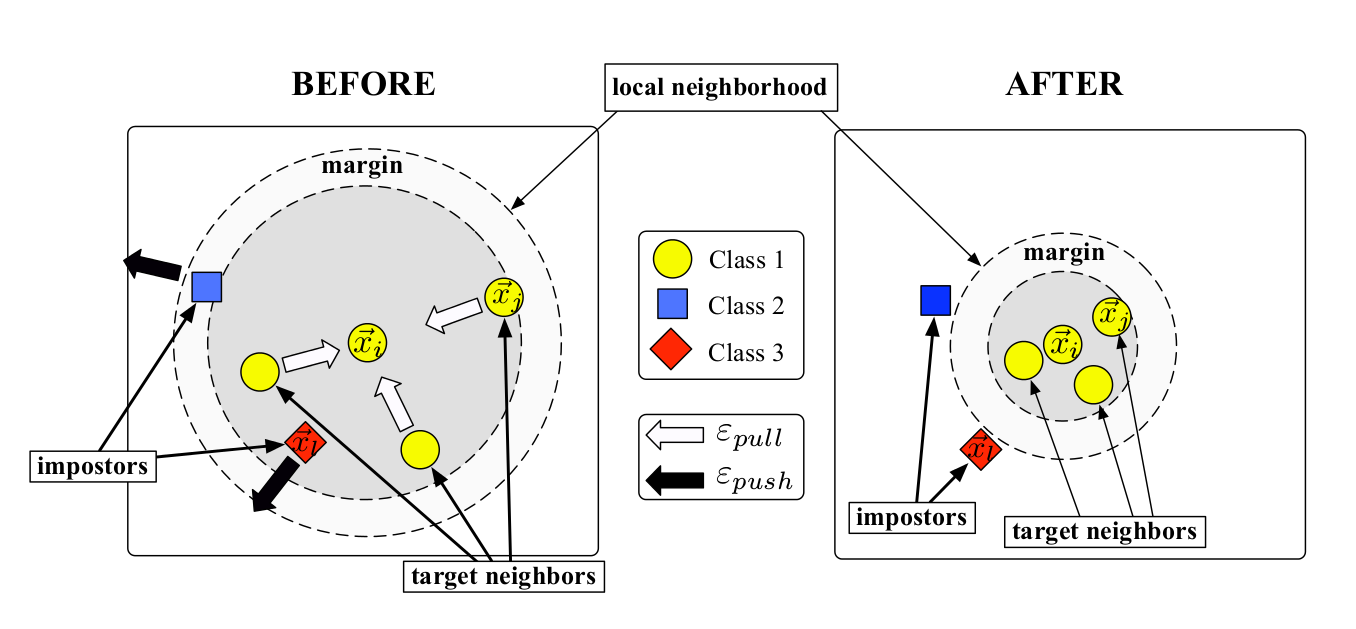
\includegraphics[width=0.9\linewidth]{schema_lmnn}
	\caption{Neighborhood of a point, from \autocite{LMNN09}.\label{fig:lmnn}}
\end{figure}
Specifically, let $N_i$ be the set of the $k$ closest neighbors of $x_i$ in the
original space which share the same class, called target neighbors. Closer
points of different class are impostors (see \autoref{fig:lmnn}
\vpageref{fig:lmnn}). The optimization pushes target neighbors close to $x_i$
while pulling away impostors. The number of active constraints is linear
rather than quadratic because only the neighborhood of each points contribute
to it. Thus the following semidefinite program can be solved efficiently:
\begin{equation*}
	\min_A \sum_{i, j\in N_i}
	\underbrace{d_A(x_i, x_j)}_\text{\emph{pull} target neighbor $x_j$ closer} +
	\underbrace{\mu \sum_{k, y_k\neq y_i} \left[ 1 + d_A(x_i, x_j) -
	d_A(x_i, x_k)\right]_+}_\text{\emph{push} impostor $x_k$ beyond target
	neighbor $x_j$}
\end{equation*}
where $[x]_+$ is the hinge-loss: $[x]_+=\max(0, x)$

The end result is a linear, global metric but there are other approaches. One
can learn multiple local metrics, or a non linear metric like
\methodname{Gradient Boosting LMNN} \autocite{GBLMNN12}. It solves a similar
optimization problem except that distances are computed in a new space,
obtained by a non linear additive mapping. This mapping is itself learned by
combining multiple regression trees of limited depth selected by gradient
boosting.

A more complete overview of metric learning is given in the survey of
\textcite{MetricSurvey13}.

\subsection{Set metric}

We discussed metrics between points but in this work, we also used distances
between set of such points.

geometric: For instance, the bottleneck distance \autocite{Bottleneck96} (the
smallest distance between pairs of farthest point), the sum of the distance of
each point to its closest neighbor, or the Hausdorff distance (the largest
distance between pairs of closest point) and its variation
\autocite{ModifiedHausdorff94}.

Assignment problem and Hungarian algorithm $O(n^4)$ and $O(n^3)$
\autocite{Hungarian57}. Transportation problem. Because these problem have min
cost flow constraints matrix, they are totally unimodular (\ie{} every non
singular sub square matrix has a determinant of $+1$ or $-1$) and thus admits
a integer solution. It may be more convenient to consider non integer supply
and demand, which leads to fractional weight and probabilistic interpretation.
For instance the modern Kantorovitch formulation of the Transportation
problem: $\underset{\gamma \in \Gamma(\mu, \nu)}{\mathrm{inf}} \int_{X\times
Y} c(x,y)\mathrm{d}\gamma(x,y)$. It is related to the Wasserstein distance of
two probability measures $\mu$ and $\nu$ of a space $M$ with
$p$\textsuperscript{th} finite moment $W_p(\mu, \nu) = \left( \underset{\gamma
\in \Gamma(\mu, \nu)}{\mathrm{inf}} \int_{M\times M}
d(x,y)^p\mathrm{d}\gamma(x,y)\right)^{\frac{1}{p}}$. $W_1$ is also called
\methodname{Earth Mover's Distance} \autocite{EMD98}.


An lower-complexity algorithm using L1 ground metric. Code is available and
they claim 100x speed up for 2D histograms \autocite{Ling2007}

The approximation is based on wavelet but the complexity is exponential with
the number of dimension so it's probably infeasible for d>6
\autocite{Shirdhonkar2008}

The assumption here is that there is upper bound on the distance between
points. They also exhibit nice speed-ups and code is available.
\autocite{Pele2009}

It computes lower and upper bounds of EMD quickly, with GPU and in parallel.
The author also claims that the distance performs better for classification
task. Code is available but looking at it and reading the paper, it seems to
work only in one dimension. \autocite{FastEMD13}

% ground metric learning for EMD? \autocite{LearnEMD14}

As hinted in \emd{} by the link between distance in Euclidean spaces and
probability spaces, we can also measure similarity between set of objects if we
describe them by probability distributions. Information theory provides us with
multiple tools to assess distance between distributions, the most well known
being the Kullback--Leibler divergence, defined in the discrete case as
\begin{equation*}
	\KL{p}{q} = \sum_i p_i\log\left(\frac{p_i}{q_i}\right) 
\end{equation*}
However, this divergence is not a metric as it is not symmetric (nor does is
satisfy the triangular inequality). Thus, we used a metric based on it, the
\methodname{Jensen--Shannon Divergence} \autocite{JensenShannon03}, which is
defined using the average $m=\frac{p+q}{2}$
\begin{equation*}
	\JSD{p}{q} = \frac{1}{2}\left(\KL{p}{m} + \KL{q}{m}\right) 
\end{equation*}
